\documentclass[a4paper,12pt]{article} %style de document
\usepackage[utf8]{inputenc} %encodage des caractères
\usepackage[french]{babel} %paquet de langue français
\usepackage[T1]{fontenc} %encodage de la police
\usepackage[top=2cm,bottom=2cm,left=2cm,right=2cm]{geometry} %marges
\usepackage{graphicx} %affichage des images
\usepackage{amssymb}
\usepackage{url}
\usepackage{verbatim}
\usepackage{amsmath}
\usepackage{color}
\usepackage{tikz}
\usepackage{hyperref}
\hypersetup{
	hidelinks,
    colorlinks,
    citecolor=black,
    filecolor=black,
    linkcolor=black,
    urlcolor=black
}

\begin{document} %début du document

%----------------------------------
%page de garde
%----------------------------------

\begin{titlepage}

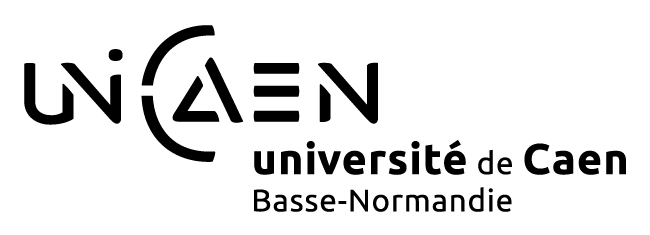
\includegraphics[scale=0.3]{images/unicaen.png}

\vspace{7cm}

\begin{center}

\begin{Huge}
Méthodes de conception\\
Rapport de Projet\\
\end{Huge}
\vspace{2cm}
\begin{large}
Beauchamp Aymeric 21301016\\
Demé Quentin 21507097\\
Jacqueline Martin 21507982\\
Zaizafoun Sami 21600538\\
\vspace{1cm}
L3 Informatique  Groupe A2
\end{large}

\end{center}
\end{titlepage}


%------------------------------
%sommaire
%------------------------------

\newpage

\tableofcontents

\newpage

%------------------------------
%contenu
%------------------------------

\section*{Présentation du projet}

L'application à développer est un jeu de stratégie au tour par tour. Chaque joueur peut se déplacer sur une grille de jeu et utiliser des armes pour vaincre ses adversaires, le but étant d'être le dernier joueur vivant.\\
Nous avons pris quelques libertés par rapport au sujet de base : chaque joueur dispose ainsi de points de vie et de points d'action, au lieu d'une simple quantité d'énergie.
Les joueurs perdent lorsqu'ils n'ont plus de points de vie, et utilisent les points d'action pendant leur tour pour effectuer leurs actions (se déplacer, tirer, utiliser le bouclier...). Les points d'action sont restitués au début du tour d'un joueur.\\
Pendant un tour, les joueurs peuvent agir autant qu'ils le veulent, tant qu'ils ont assez de points d'action pour le faire. Le tour d'un joueur se termine quand il n'a plus de points d'actions ou quand il décide de passer sans dépenser ce qui lui reste.

\section*{Organisation du code}

L'application est séparé en deux packages : le package modele qui contient tout ce qui est nécessaire au fonctionnement du jeu, et le package graphics qui permet l'utilisation du jeu en interface graphique.

\begin{figure}[!h]
\centering
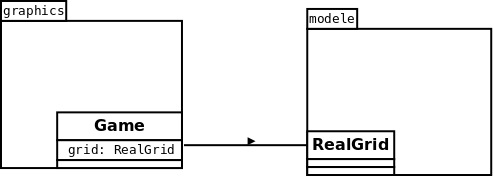
\includegraphics[scale=0.5]{images/packages.png}
\caption{Diagramme de packages}
\end{figure}

\begin{figure}[!h]
\centering
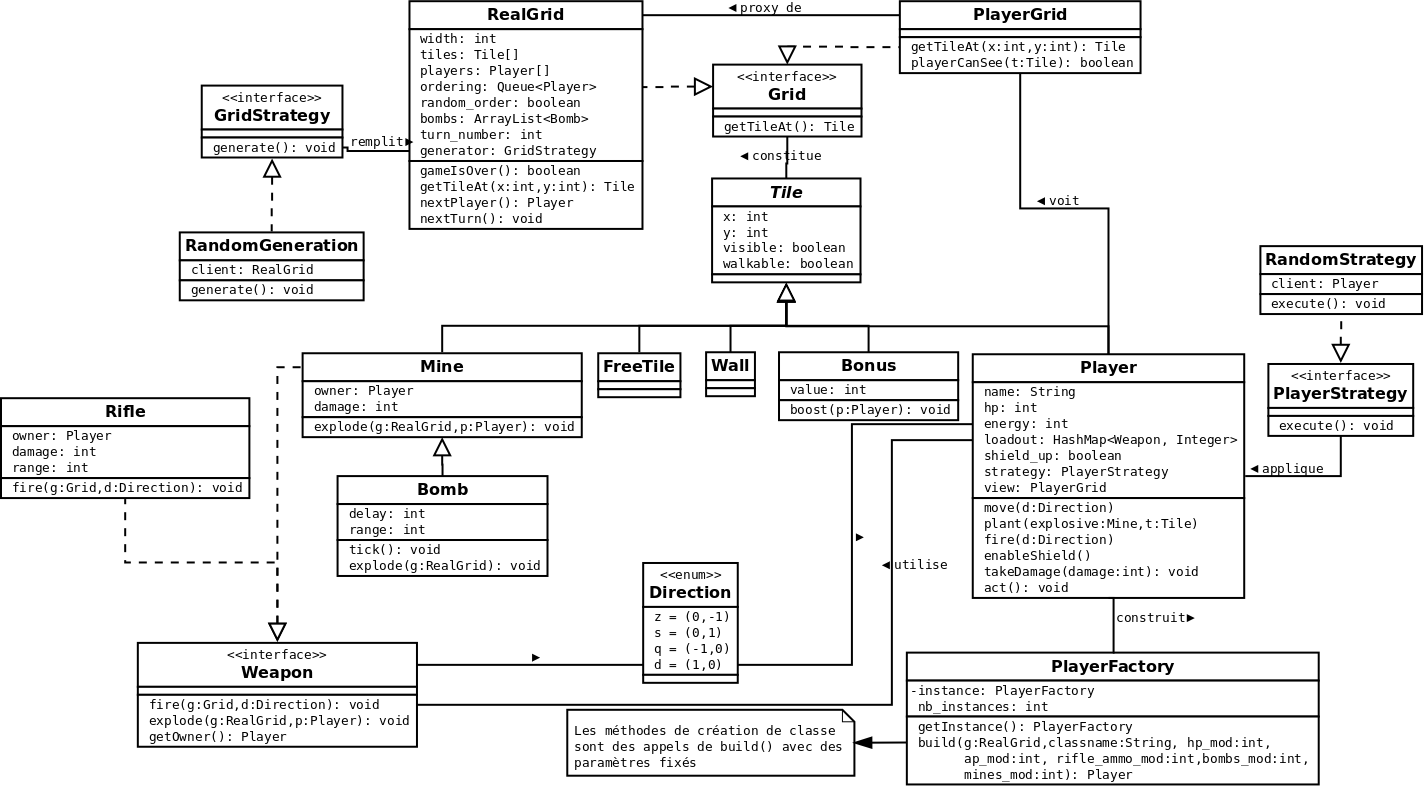
\includegraphics[scale=0.33]{images/modele.png}
\caption{Diagramme de classe du package modele}
\end{figure}
\end{document}

